\documentclass[12pt, a4paper, twoside]{article}
\usepackage[utf8]{inputenc}
% font size could be 10pt (default), 11pt or 12 pt
% paper size coulde be letterpaper (default), legalpaper, executivepaper,
% a4paper, a5paper or b5paper
% side coulde be oneside (default) or twoside 
% columns coulde be onecolumn (default) or twocolumn
% graphics coulde be final (default) or draft 
%
% titlepage coulde be notitlepage (default) or titlepage which 
% makes an extra page for title 
% 
% paper alignment coulde be portrait (default) or landscape 
%
% equations coulde be 
%   default number of the equation on the rigth and equation centered 
%   leqno number on the left and equation centered 
%   fleqn number on the rigth and  equation on the left side
%	
\author{Sven Fiergolla}
\title{Universelle Turingmaschine mit zwei Zuständen/Symbolen}
\date{\today}

\begin{document}
 
\maketitle


\section{Einführung}
\subsection{Informelle Definition der Turingmaschine}
%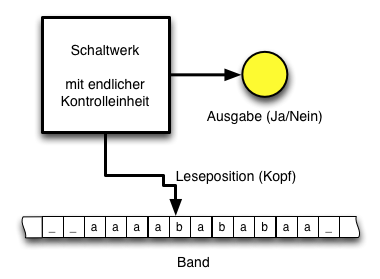
\includegraphics[scale=1]{TMKonzept.png}
Turingmaschinen (im folgenden TM), benannt nach \textit{Alan M. Turing}, sind das allgemeine Modell der theoretischen Informatik.
Sie bestehen aus einem \textit{unendlichen Band}, welches die Eingabe beinhaltet, einem \textit{Lese/Schreibkopf} welcher eine eindeutige Position auf dem Band hat und einem \textit{Steuerungselement}, häufig beschrieben durch eine (partielle) Übergangsfunktion.


\subsection{Formale Definition der Turingmaschine}
Formal wir die Turingmaschine als Septupel $\mathbf{ M = (Q,\Sigma,\Gamma,\sigma} $


\subsubsection{even more introduction}
come to the point \ldots

\paragraph{Paragraphs}
A paragraph is small but 

\subparagraph{Subparagraphs}
subparagraphs are smaller! 

\paragraph{Outline}
First we start with a little example of the article class, which is an 
important documentclass. But there would be other documentclasses like 
book \ref{book}, report \ref{report} and letter \ref{letter} which are 
described in Section \ref{documentclasses}. Finally, Section 
\ref{conclusions} gives the conclusions.



\section{Documentclasses} \label{documentclasses}

\begin{itemize}
\item article
\item book 
\item report 
\item letter 
\end{itemize}


\begin{enumerate}
\item article
\item book 
\item report 
\item letter 
\end{enumerate}

\begin{description}
\item[article\label{article}]{Article is \ldots}
\item[book\label{book}]{The book class \ldots}
\item[report\label{report}]{Report gives you \ldots}
\item[letter\label{letter}]{If you want to write a letter.}
\end{description}

\section{tabular}
No paper without a tabular!

\begin{tabular}{|l|c|r|p{2cm}|}
\hline
first column & second column & third column & fourth column \\
\hline 
l stand for left & c for center & r for right & and p for predefined size \\
\hline 
\end{tabular} 


\section{some math}

Math in text is called in line math just put \$ character around 
the math think. Like $ a^2 + b^2 = c^2 $. It looks better if you use 
this 
\[a^2 + b^2 = c^2\]

\section{Conclusions}\label{conclusions}
There is no longer \LaTeX{} example which was written by \cite{doe}.

\begin{thebibliography}{9}
\bibitem[Doe]{doe} \emph{First and last \LaTeX{} example.},
John Doe 50 B.C. 
\end{thebibliography}

\end{document}
